\documentclass{article}
\usepackage{tikz}
\usetikzlibrary{automata}
\usetikzlibrary{arrows}

\begin{document}

\begin{center}
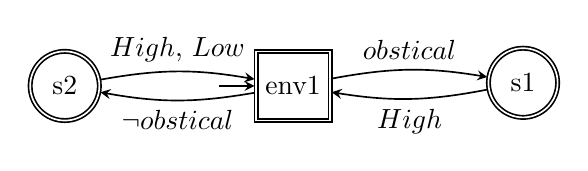
\begin{tikzpicture}[
  auto,
  initial text=,
  semithick,
  >=stealth,
  ,
  p0/.style={circle},p1/.style={rectangle}
]
  \node[state,accepting,p0](s1) at (3.04,1.04){s2};
  \node[state,initial,accepting,p1](s2) at (5.94,1.04){env1};
  \node[state,accepting,p0](s3) at (8.86,1.08){s1};
  \path[->]
    (s1) edge [bend left=10] node {$High$,\ $Low$} (s2)
    (s2) edge [bend left=10] node {$\neg obstical$} (s1)
    (s2) edge [bend left=10] node {$obstical$} (s3)
    (s3) edge [bend left=10] node {$High$} (s2)
  ;
\end{tikzpicture}
\end{center}
\end{document}
